% 2014 Shanghai liberal Q17: 2x2 small squares forming one big square; 9 labeled lattice points.
% All segments solid, no arrows; dots at every vertex used by the figure.
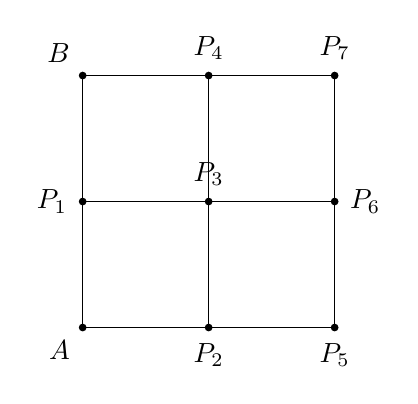
\begin{tikzpicture}[line width=.6pt, font=\normalsize]
\tikzset{d/.style={circle, fill, inner sep=0pt, minimum size=2.8pt}}
\def\u{1.6}
\coordinate (A) at (0,0);
\coordinate (P2) at (\u,0);
\coordinate (P5) at (2*\u,0);
\coordinate (P1) at (0,\u);
\coordinate (P3) at (\u,\u);
\coordinate (P6) at (2*\u,\u);
\coordinate (B) at (0,2*\u);
\coordinate (P4) at (\u,2*\u);
\coordinate (P7) at (2*\u,2*\u);
\draw (A) -- (P5);
\draw (P1) -- (P6);
\draw (B) -- (P7);
\draw (A) -- (B);
\draw (P2) -- (P4);
\draw (P5) -- (P7);
\foreach \p in {A,P1,P2,P3,P4,P5,P6,P7,B} {\node[d] at (\p) {};}
\node[below left=1pt] at (A) {$A$};
\node[below=2pt] at (P2) {$P_{2}$};
\node[below=2pt] at (P5) {$P_{5}$};
\node[left=2pt] at (P1) {$P_{1}$};
\node[above=2pt] at (P3) {$P_{3}$};
\node[right=2pt] at (P6) {$P_{6}$};
\node[above left=1pt] at (B) {$B$};
\node[above=2pt] at (P4) {$P_{4}$};
\node[above=2pt] at (P7) {$P_{7}$};
\end{tikzpicture}
